\documentclass[a4paper, 12pt]{scrartcl}
\usepackage[utf8]{inputenc}
\usepackage[ngermanb]{babel}
\usepackage{setspace}
\usepackage{geometry}
\usepackage{graphicx}
\usepackage{cite}
\usepackage{amsmath}
\geometry{a4paper, top=25mm, left=25mm, right=25mm, bottom=25mm}

\title{Seminar IT-Sicherheit}
\author{Kevin Seidel \\ Studiengang Informatik \\ Matrikelnummer: 943147}

\begin{document}
\begin{titlepage}
\begin{center}
\vspace*{1.5cm}
\begin{Large}
\textbf{Universität Osnabrück}
\end{Large}

\noindent\hrulefill
\\[3.5cm]
PRAKTIKUMSBERICHT \\[1cm]
zum Programmierpraktikum \\[1cm]
\textbf{Paralelle Algorithmen mit OpenCL} \\[1.5cm]
im Sommersemester 2013 \\[1.5cm]
Thema: \\[0.5cm]
\textbf{Voxelization} \\[2cm]
Erstellt am 15.10.2013
\end{center}
\vfill
\begin{flushleft}
Vorgelegt von: 
\hfill \parbox{46mm}{Kevin Seidel} \\
\hfill \parbox{46mm}{943147} \\
\hfill \parbox{46mm}{Falkenstra"se 43} \\
\hfill \parbox{46mm}{49124 Georgsmarienh"utte}
\end{flushleft}
\end{titlepage}

\newpage

\pagenumbering{Roman}
\setcounter{page}{2}
\tableofcontents

\newpage
\pagenumbering{arabic}
\setcounter{page}{1}

\section{Einleitung}
W"ahrend des Praktikums habe ich mich mit der Voxelization von Szenen auf der GPU besch"aftigt. 

\section{Voxel und Voxelization}
\subsection{Voxel}
Das Wort Voxel setzt sich aus den englischen Begriffen ''volumetric'' und ''pixel'' zusammen. Frei "ubersetzt kann man es als einen dreidimensionalen Pixel bezeichnen.
Das Voxel hat im Allgemeinen nur zwei Eigenschaften, welche dem eines Pixels gleichkommen. Es besitzt eine Position in einem vorher festgelegtem dreidimensionalem Raum und einen Farbwert.
F"ur meinen Verwendungszweck wird das Voxel als W"urfel dargestellt, wobei alle Seiten die Farbe des Voxels tragen.
\subsection{Voxelization}
Die Voxelization ist die "Uberf"uhrung einer Szene aus Polygonen in Voxel. Diese Aufgabe kann hochgradig paralell ausgef"uhrt werden, wodurch sich die Nutzung der GPU f"ur dieses Verfahren anbietet. In der Literatur zu diesem Problem gibt es mehrere L"osungsans"atze. In fr"uheren Arbeiten wurde die Szene in mehrere Ebenen eingeteilt, sodass jede Voxelebene seperat gerendert wurde. Dies f"uhrt dazu, dass diese Verfahren sehr langsam ist, da f"ur h"ohere Dimensionen sehr viele Renderaufrufe durchgef"uhrt werden m"ussen.

Eine etwa neuere Taktik nutzt die Paralellisierbarkeit dieser Aufgabe aus und "uberpr"uft Kollisionen zwischen den Polygonen und den Voxeln mittels GPU-Computing. Dieser Ansatz kann sowohl mittels Cuda als auch mittels OpenCL gel"ost werden. Im weiteren Verlauf dieser Arbeit wird nur der Ansatz mittels OpenCL dargelegt.
Bei dieser neueren Methode wird f"ur jedes Polygon in der Szene ein eigener Thread gestartet und innerhalb dieses Threads wird "uberpr"uft, ob das Polygon ein Voxel "uberschneidet. Das Ergebnis wird dann in einen Buffer geschrieben, welcher dann f"ur jede Stelle des Voxelgrids einen Wert enth"alt, welcher angibt, ob das Voxel gef"ullt ist oder nicht.

\section{Voxelization mit Hilfe von OpenGL}
Zuerst habe ich mich mit der Voxelization mittels OpenGL besch"aftigt. Dieser Ansatz ist eine neuere Methode, da hierbei Funktionen aus OpenGL 4.2 genutzt werden. Diese Version erschien im August 2011. 
Der OpenGL-Ansatz nutzt hierbei die feste Hardware-Pipleline der Grafikkarte aus, um den Prozess der Voxelization zu beschleunigen. Hierbei wird im spezifischen der Hardware-Rasterizer genutzt, um die "Uberschneidung der Polygone und der Voxel zu bestimmen. 

Ein Problem, welches hierbei auftaucht, ist, dass der Rasterizer dar"ur gedacht ist, eine zwei-dimensionale Szene zu rastern. F"ur das hier vorliegende Problem muss jedoch eine dreidimensionale Szene gerastert beziehungsweise voxelisiert werden.
Um dieses Problem zu l"osen, werden die Polygone vor der Rasterisierung, in Richtung der dominanten Achse ihrer Normalen projeziert. Hierdurch wird die gr"o"st m"ogliche Fl"ache des Dreiecks rasterisiert. Nach der Rasterisierung hat man nun die vom Polygon "uberschnittenen Pixel erfasst. Um diese nun in Voxel zu "uberf"uhren, werden die Pixel zur"uck projeziert, sodass sie sich nun im dreidimensionalen Raum befinden.

\begin{figure}
	\centering
		\includegraphics[width=16cm]{Voxelization-Pipeline}
	\caption{Schritte der Voxelization mittels OpenGL}
\end{figure}

Die entstehenden Voxel werden dann mittels der in OpenGL 4.2 eingef"uhrten Methode ''image-write'', welche es erlaubt, im Fragment-Shader, an eine beliebige Stelle in einer Textur zu schreiben, in eine 3D-Textur geschrieben. Hierbei wird die Position des Voxels und dessen Farbwert geschrieben.


Mittels dieser Textur lassen sich die Voxel nun problemlos ausgeben. Es ist also m"oglich zu "uberpr"ufen, ob ein Voxel vorhanden ist und welche Farbe er besitzt.

Eine Schw"ache dieser Methode ist, dass es vorkommen kann, dass auf Grund der n"otigen Projektion einige Voxel nicht registriert werden. Dies ist darauf zur"uckzuf"uhren, dass "Uberschneidungen nur am Mittelpunkt des Pixel getestet werden. Hierf"ur existiert jedoch eine L"osung: 

Das zu testende Polygon wird so vergr"o"sert, dass das vorherige Polygon, welches einen Pixel nur ber"uhren w"urde, nun den Mittelpunkt "uberschneidet. 



\section{Voxelization mit Hilfe von OpenCL}
Bei der Voxelization mittels OpenCL muss die Erkennung von "Uberschneidungen individuell programmiert werden, da hier nicht auf einen feste Pipeline zur"uckgegriffen werden kann. Dies erlaubt jedoch auch mehr Freiheiten bei der Erkennung, Verarbeitung und Speicherung der Voxeldaten. 

Bei der "Uberf"uhrung von Polygonen in Voxel mittels eines OpenCL-Kernels wird f"ur jedes Polygon der zu voxelisierenden Szene ein eigener Thread gestartet, sodass alles Polygone paralell bearbeitet werden. In jedem Kernelaufruf wird daf"ur auf die "Uberschneidung zwischen dem jeweiligen Polygon und den Voxeln getestet. Um diesen Vorgang zu beschleunigen, wird nur in der in Frage kommenden Bounding-Box des aktuellen Dreiecks getestet.
Das hei"st, es werden die Eckpunkte einer Box berechnet, welche das Dreieck umschlie"sen w"urde. Dadurch muss nicht die komplette Szene auf "Uberschneidungen getestet werden, sondern nur ein kleinerer Ausschnitt.

F"ur jedes Voxel wird nun getestet, ob sich ein oder mehrere Eckpunkte auf verschiedenen Seiten eines Polygons befinden. Dadurch werden die Voxel bestimmt, welche sich an den Kanten der Polygone befinden. 

\begin{figure}
	\centering
		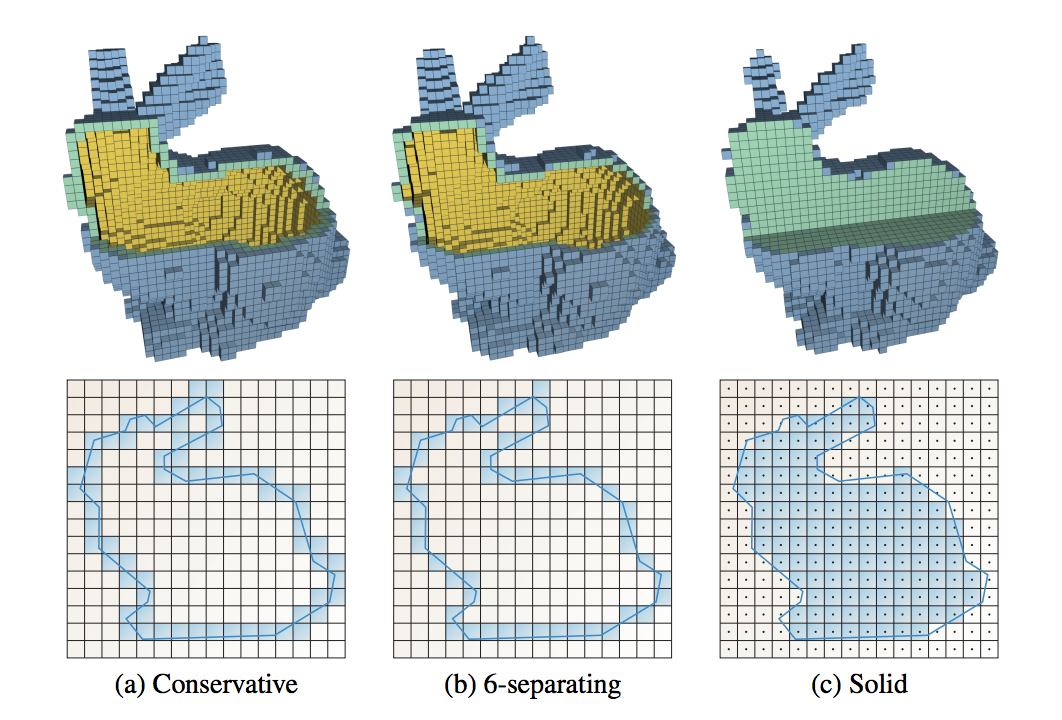
\includegraphics[width=16cm]{Kinds-of-Voxelization}
	\caption{Verschiedene Arten der Voxelization}
\end{figure}

Des Weiteren wird "uberpr"uft, ob sich die 2D-Projektion des Polygons und des Voxels "uberlappen. 

Wenn beide Tests eine "Uberschneidung best"atigen, ist eine "Uberschneidung best"atigt und kann so geschrieben werden.
Die Speicherung der Voxel ist bei diesem OpenCL Ansatz frei w"ahlbar. 
In meinem Ansatz wurden alle Voxel in einen eindimensionalen Buffer geschrieben. 

\begin{figure}
		$Buffer: (x0, y0, z0), (x0, y0, z1), ..., (x0, y0, z511), (x0, y1, z0), ..., (x511, y511, z511)$
\caption{Aufbau des Buffers f"ur ein Voxelgrid der Dimension $512^3$}

\end{figure}

\section{Vergleich zwischen OpenGL und OpenCL Ansatz}

\section{Speicherung der Voxeldaten}
Um die Nutzung zu beschleunigen und den Speicherbedarf gering zu halten, werden die Voxel in Sparse Octrees gespeichert. 
Das hei"st, dass gr"o"sere zusammenh"angende Fl"achen des gleichen Typs beziehungsweise der gleichen Farbe, nicht in kleinere Teile zerlegt werden, da dies nicht n"otig ist.
Dadurch l"asst sich zum Beispiel bei Szenen, welche nur sp"arlich gef"ullt sind, viel Speicherplatz sparen. 
Auch die Verarbeitungszeit verbessert sich, da im resultierenden Octree f"ur diese speziellen Fl"achen nicht so weit in die Tiefe des Baumes geschaut werden muss.

\section{Nutzung der Voxeldaten}
Nach der Erzeugung der Voxeldaten stellt sich nat"urlcih die Frage, was nun damit gemacht wird. 
Die Voxel sollen f"ur ein Beleuchtungsmodell verwendet werden. Im Genaueren wird mittels der Voxeldaten die indirekte Beleuchtung errechnet.
Dabei wird das Voxel Cone Tracing verwendet, welches einem vereinfachten und simplerem Raytracing entspricht.
Hierbei wird nicht , wie beim klassischen Raytracing, f"ur jeden Bildpunkt ein Strahl in die Szene geschossen, sondern ein Kegel, welcher in naher Distanz relativ hochaufl"osend ist, f"ur weiter entfernte Berechnungen jedoch nur eine N"aherung liefert. Durch die Nutzung eines Octrees in der Speicherung der Daten, ist diese Methode bedeutend schneller als das klassischen Raytracing, da deutlich weniger Daten verarbeitet werden m"ussen. 

\section{Ausblick und Fazit}
Mit heutiger Hardware ist ein Echtzeit-Raytracing einer komplexen Szene und zu einer brauchbaren Bildrate noch nicht m"oglich. Die von mir vorgestellte Methode, bestehend aus Voxelization, der Sparse Voxel Octree-Speicherung und des Voxel Cone Tracing, k"onnen auf heutiger Hardware schon zufriedenstellende Beleuchtungsergebnisse und Bildraten erzielen. 
Daher ist dieser Ansatz f"ur die n"ahere Zukunft sehr vielversprechend, da auch bei steigenden Aufl"osungen der Szenen noch zufriedenstellende Ergebnisse erzielt werden k"onnen, wohingegen das Raytracing mit der heute zug"anglichen und auch zuk"unftigen Hardware noch einige Jahre brauchen wird, bis es f"ur die Echtzeitdarstellung von 3D-Szenen genutzt werden kann, da hierf"ur eine deutlich schnellere Grafikhardware von N"oten ist.

\end{document}